% vi: filetype=tex
% Chapter 3
%TODO - Let's first describe all examples heurestically, then define the
%dimensions, give examples where they are not equal, then analyse cantor set as
%a strange set.

\chapter{Fractals : An Overview} % Main chapter title and the space will
%fucking remain here just cuz

\label{Chapter3} % For referencing the chapter elsewhere, use \ref{Chapter3} 

\lhead{Chapter 3. \emph{Fractals}} % This is for the header on each page - perhaps a shortened title

\section{Introduction and Overview}
Fractals, a term now popular, was coined relatively recently (1975, by Benoit
Mandelbrot) while investigating the `roughness' of nature; in his own words.
It was chosen along the intuition that these objects somehow possess fractional
, fragmented properties.
\newline
But nature or its investigation isn't where these objects received their first
formal recognition, it was in the investigations of pure mathematics. The first
formally studied objects having 'fractal'-like properties were the Cantor set of
middle-thirds, space-filling curves like Peano's and Hilbert's,
everywhere continuous but nowhere differentiable function etc. These date as far
back as the end of the 19th century : a time of revolution in mathematics. 
At the time, these constructions of men
were unwelcome and pathological examples which deviated from the standard in
mathematics, nor were they inspired by nature it had
seemed and hence were gilded with
the term `monster' curves.\cite{mandelbrot}
\newline
Benoit Mandelbrot, as mentioned earlier, was studying the irregularities in
nature and the topics were wide and diverse. One of the aims were to quantify
the irregular shapes and surfaces often found in the physical world
and to bring some semblance of sense and order. Some examples in nature like
brownian motion, coastlines etc had been individually studied. But Mandelbrot
brought them under the single banner of fractals, along with the mathematical
curves mentioned. Then he used already developed areas like the Hausdorff
Dimension to successfully make sense of fractals. Many other contributions were
made and presented in the form of the book `Fractal Geometry of Nature'. These
contributions included both the understanding of fractals, and then subsequent
use and application to very interesting answer questions in mathematical
sciences. The most important area of application was perhaps to the study of
what's traditionally called `chaos'. And hence the field of Fractal Geometry
entered mainstream research and still continues to be an active area.
\newline One important aspect of all fractals that derserves special emphasis is
that they ward off all attacks of classical geometry and demand new approaches
to make sense of and understand geometrically.\cite{mandelbrot}


\section{Examples and Features}
This section provides visual examples to get acquainted with fractals.
\subsection{Fractals From Math}
\subsubsection{Cantor Set}
\begin{figure}[h!]
    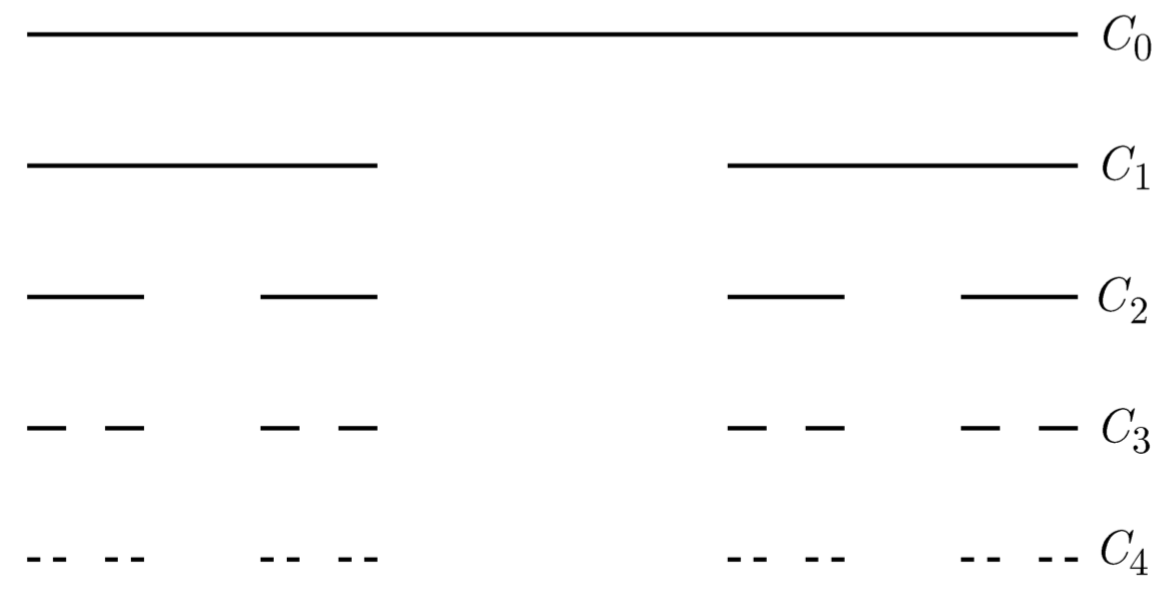
\includegraphics[width=\linewidth]{Pictures/cantor_set.png}
    \caption{First four iterations of Cantor Set.}
    \label{fig:cantor_set}
\end{figure}
Cantor set is arguably the most important fractal one could consider, and also
the simplest in terms of set theory. 
\begin{definition}
    Cantor set is defined as\cite{edgar}
    \[
        C = \bigcap_{i=0}^{\infty} C_i
    \]
    where  
    \[
        C_0 = [0,1]
    \]
    \[
        C_1 = [0,\frac{1}{3}] \cup [\frac{2}{3}, 1]
    \]
    \[
        C_2 = [0, \frac{1}{9}] \cup [\frac{2}{9}, \frac{3}{9} \cup
        [\frac{6}{9}, \frac{7}{9}] \cup [\frac{8}{9}, 1]
        \]
        \[
            \vdots
        \]
        are iteratively constructed by removing the middle third of every interval
        and retaining the rest in every iteration.
\end{definition}
\subsubsection{Koch Curve}
\begin{figure}[h!]
    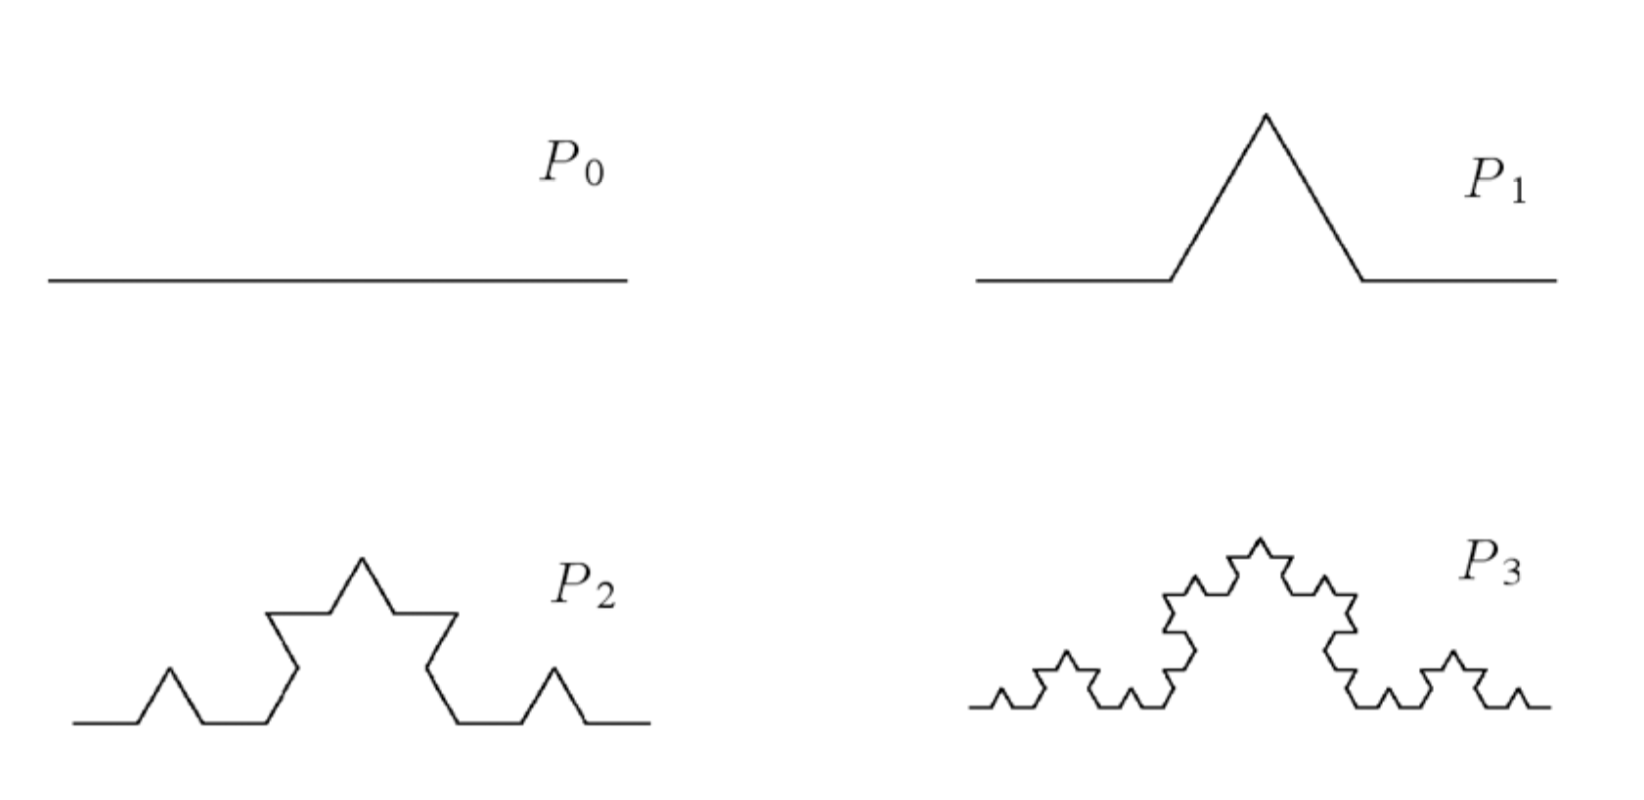
\includegraphics[width=\linewidth]{Pictures/koch_curve.png}
    \caption{Koch Curve.}
    \label{fig:cantor_set}
\end{figure}
\begin{figure}[h!]
    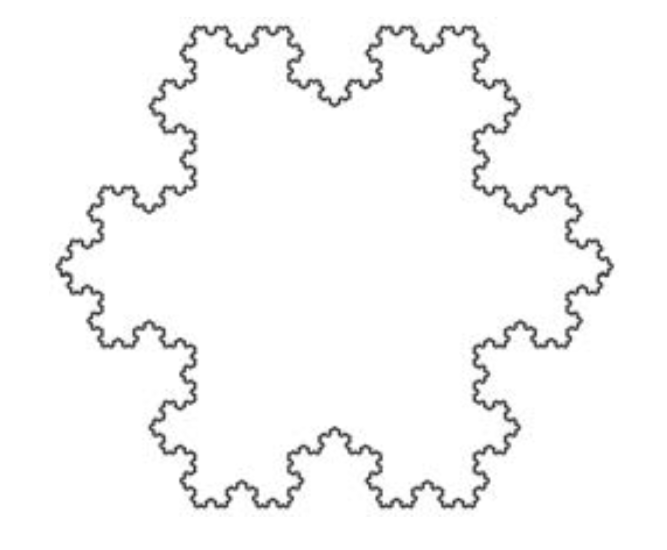
\includegraphics[width=\linewidth]{Pictures/snowflake.png}
    \caption{Snowflake made from Koch curves.}
    \label{fig:snowflake}
\end{figure}
Koch curve was first described in 1904 by von Koch as a continuous but nowhere
differentiable curve, which could constructed simply.
The Koch Snowflake has infinite length like the Koch curve, but has finite area.

The curve can be constructed in multiple ways, one of them being starting with
a line segment. Then construct an equilateral triangle with the middle third of
the line segment. Then the part of the trianlge coinciding with the orginal
segment is truncated. This way we get the next iteration, $P_1$. Repeating the
same with every line segment, we get $P_2$. Koch curve is said to be the
limiting iteration and n tends to $\infty$.

\subsection{Fractals in Nature}
\subsubsection{Physical Objects Resembling Fractals}
\begin{figure}[h!]
    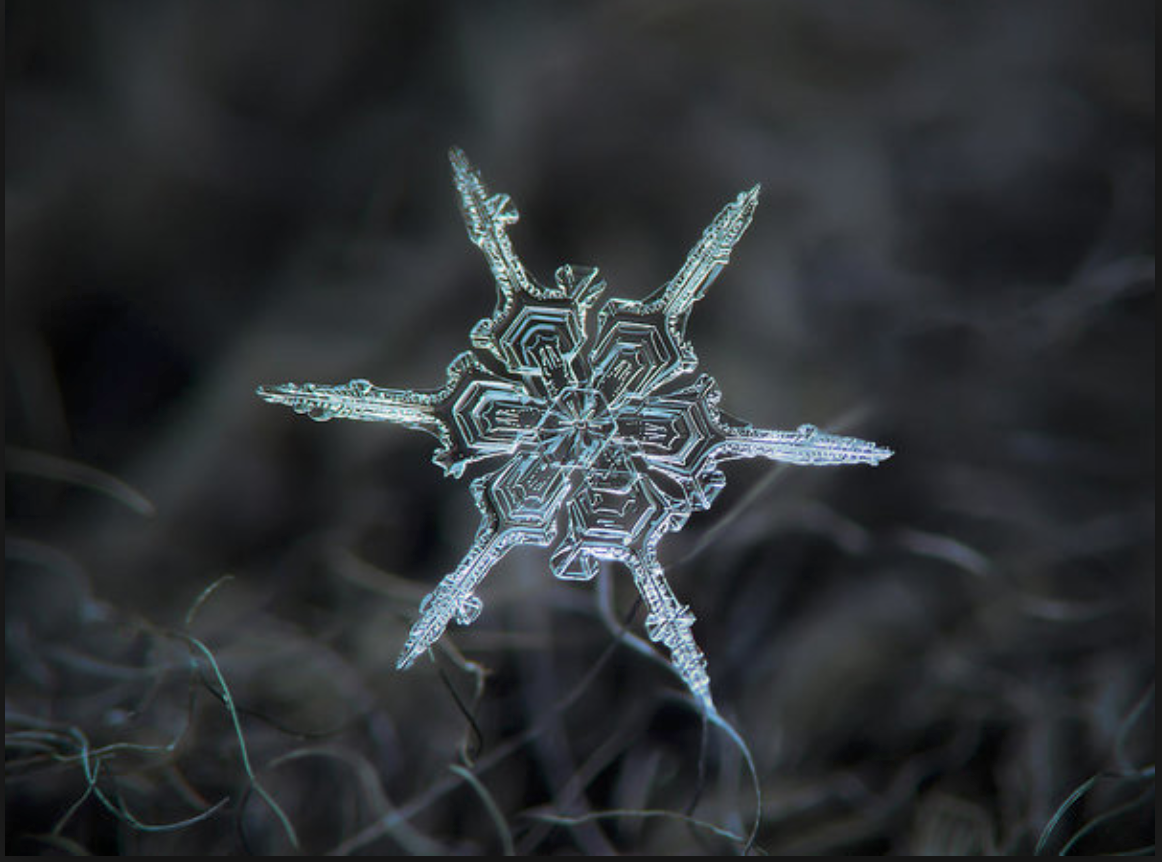
\includegraphics[width=\linewidth]{Pictures/real_snowflake.png}
    \caption{A real snowflake.}
    \label{fig:real_snowflake}
\end{figure}
\begin{figure}[h!]
    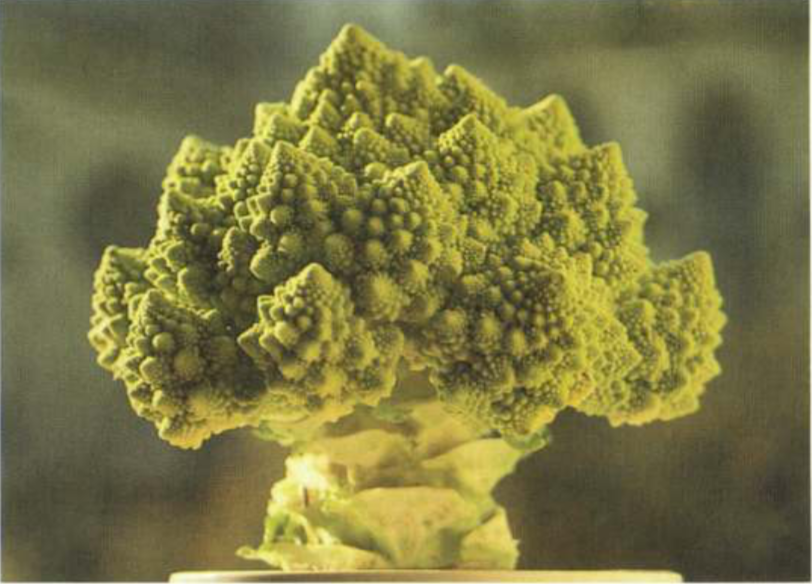
\includegraphics[width=\linewidth]{Pictures/broccoli.png}
    \caption{Broccoli.}
    \label{fig:broccoli}
\end{figure}
\begin{figure}[h!]
    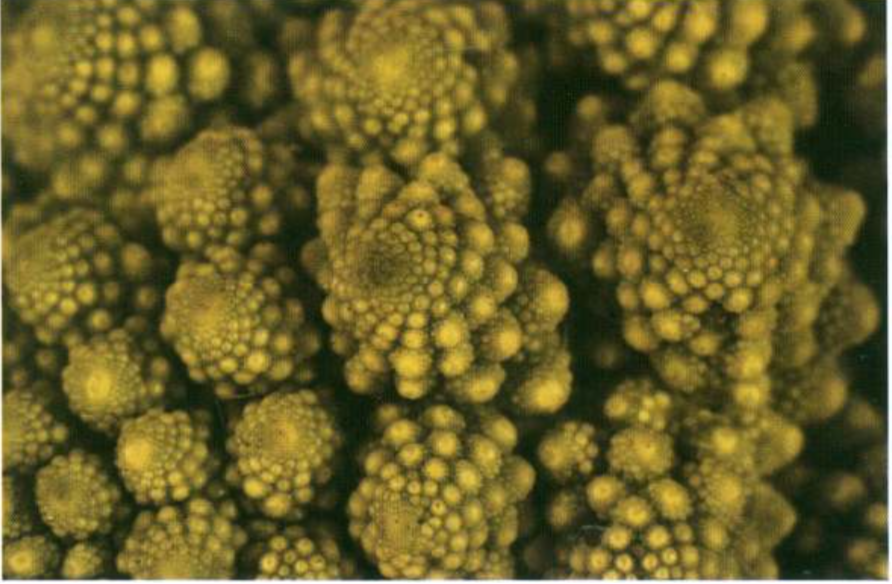
\includegraphics[width=\linewidth]{Pictures/broccoli_zoomed.png}
    \caption{Broccoli's scaling.}
    \label{fig:broccoli_zoomed}
\end{figure}
Some physical objects like the surface of a mountain, the coastline, the surface
of a broccoli etc are 'rough' and non-euclidean in nature. They are better
modeled for desired properties as fractals due to their self-similarity. The
Koch snowflake is called so because it resembles a real snowflake.
\subsubsection{Other Occurences}
\begin{figure}[h!]
    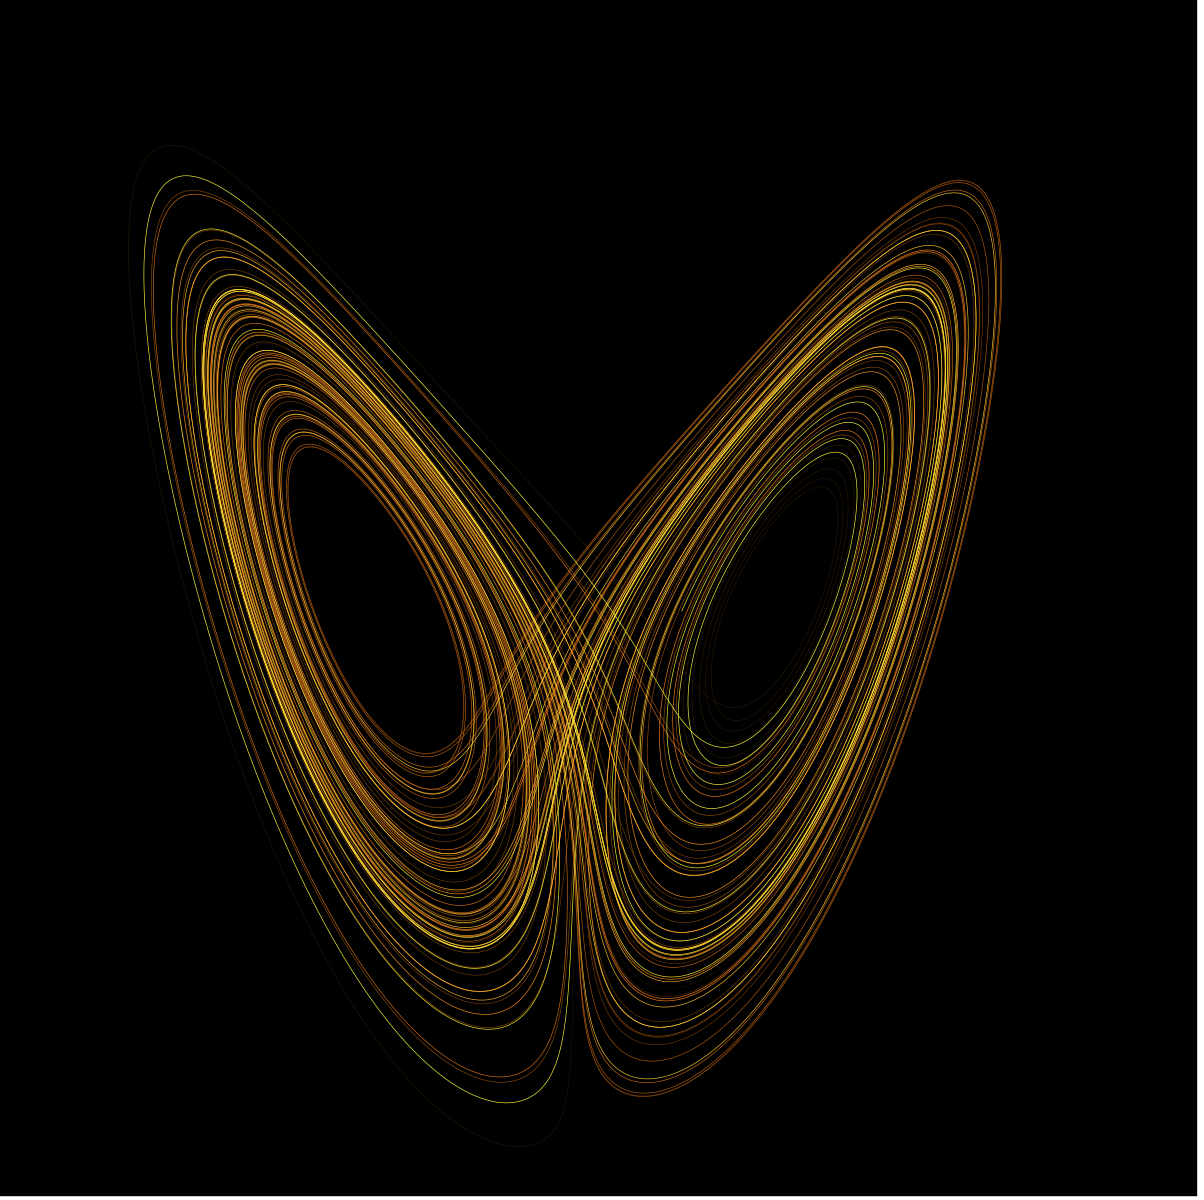
\includegraphics[width=\linewidth]{Pictures/strange_attractor.png}
    \caption{Strange attractor for Lorenz Equations.}
    \label{fig:strange_attractor}
\end{figure}
As mentioned before, fractals have been successfully used to model a wide
variety of things in nature, either directly or indirectly. Indirectly, fractals
have played a very crucial role in study of dynamical systems. Simple non-linear
dynamical systems like a double pendulum show high sensitivity to initial
conditions. What this means is that for the same pendulum, two mildly different
initial points can lead to two wildly different end points. What's interesting
is that the resulting sets are extremely erratic at first glance, but they often
turn out to be fractals. In these cases, they are called strange
attractors.\cite{strogatz}
For example, consider the Lorenz System$(\rho = 28, \sigma =10,
\beta=\frac{8}{3})$ and it's solution plot as shown in
\ref{fig:strange_attractor},
\[
    \frac{dx}{dt} = \sigma(y - x)
\]
\[
    \frac{dy}{dt} = x(\rho -z) - y
\]
\[
    \frac{dz}{dt} = xy - \beta z
\]

\subsection{Heurestic Features}
A pre-requisite to defining something is the identification of its properties.
Objects which have come to be alluded to as fractals often possess the following
properties, as defined in natural language
\begin{enumerate}
    \item Defined simply : This only means that usually a recursive method of
        definition is provided which is simple to state. Simplicity in being
        stated doesn't go controrary to the complexity that is generated on
        following those steps of recursive generation.
    \item Fine Structure or Scaling : This means that fractals possess detail at
        all
        scales. In other words, in the classical geometry...the more you zoom in
        to a point, the more smooth it becomes. But this is simply not true for
        fractals. Zooming in doesn't lead to any loss in local detail. Nor does
        zooming out lead to a loss of global detail.
    \item Self-Similarity : Fractals usually possess self-similarity in one form
        or another at different scales. What this means is that they exhibit
        repeating patterns at different scales.
    \item Non-standard Behaviour : 
        They are too irregular a collection of points in a Euclidean space to
        be studied through the tools of classical or Euclidean geometry.
\end{enumerate}


\section{Mathematics of Fractals}
Studying fractals mathematically is an area of active research. Consensus on
what should be called a fractal or what shouldn't hasn't yet been reached in
absolution. Hence the field currently consists of tools and tricks for analysing
different structures using different methods.
\newline The study and analysis for fractals and their geometry
takes multiple hints from the
approach of classical geometry, even though its methods are NOT applicable.
These include study of global properties using various notions of dimension,
study of local behaviour of fractals, projections, intersections etc.
\newline Even though an all encompassing definition is not yet available,
analysis can only proceed through definition. Following definition includes
most
objects deemed fractals and only skips few borderline cases, is the best
available mathematical definition and hence will be used.
\begin{definition}
    A subset of a Euclidean space $\bm{R}^n$ is called a fractal if its
    hausdorff dimension is strictly greater than its topological dimension.
\end{definition}
The terms will be defined in the following sections.

\subsection{Covering or Topological Dimension}
The idea behind the covering dimension is that one dimensional objects in
metric spaces can be `covered' with open balls which intersect with at most
one other open ball. Similarly two-dimensional objects can be covered in a
metric space using open intervals that intersect at most two other open
balls. This of course stems from experience with objects in Euclidean spaces.
\begin{definition}
    For any collection of set A in a metric space (X,d), B is called its
    refinement if it's an open cover of X such that $\forall S_A \epsilon A,
    \exists S_B \epsilon B$ such that $ S_B \subseteq S_A$.
\end{definition}
\begin{definition}
    Closed-open partition of a metric space (X,d) is an open cover of X
    consisting of disjoint sets which are all both closed and open.
\end{definition}
\begin{definition}
    A metric space is called zero-dimensional if every finite open cover has a
    finite refinement that is a closed open partition.
\end{definition}
This definition intends to make dimension an implicit property of a metric
space, so that it becomes independent of the spaces it can be embedded in.
Generalising these notions, we get
\begin{definition}
    A collection of sets is defined to have order n if the intersection of any
    number of sets greater than or equal to n+2 is a null set.
\end{definition}
\begin{definition}
    A metric space (X,d) is said to have a covering dimenion of $\leqslant$n if
    every finite open cover of X has a refinement of order $\leqslant$n. The
    covering dimension is exactly n for X if it is $\leqslant$n but not
    $\leqslant$n-1.
\end{definition}
Covering dimension is also called lebesgue dimension or topological dimension.

\subsection{Hausdorff-Besicovitch Dimension}
The Hausdorff Measure introduced in the previous chapter leads to a notion of
dimension, because of the way Hausdorff measure behaves.

\begin{theorem}
    Let $F \epsilon \bm{B(R^n)}$ and let $0 < s < t$, then
    \begin{enumerate}
        \item If $H^s(F) < \infty$, then $H^t(F) = 0$.
        \item If $H^t(F) > 0$, then $H^s(F) = \infty$.
    \end{enumerate}
\end{theorem}
\begin{proof}
    \begin{enumerate}
        \item We get from \ref{thm_haus_mea_lim},
            \[
                H^t_\delta(F) \leqslant \delta^{t-s}H^s_\delta(F)
            \]
            Limiting delta to zero, we get the answer.
        \item Similar method.
    \end{enumerate}
\end{proof}
This indicates the existence of the following 'turning' point,
\begin{definition}
    The critical value $s_0$ for Hausdorff measure such that
    \[
        H^s(F) = \infty, \: s<s_0
    \]
    \[
        H^s(F) = 0, \: s_0 < s
    \]
    is called the Hausdorff Dimension of a set F and denoted by $dim_H(F)$.
\end{definition}

The notion of this dimension was first introduced by Felix Hausdorff in 1920 in
a different context, to generalise the dimension of an inner-product space. But
it has found application for 'measurement' in unexpected places like fractals,
for which it was further developed.

%\section{Example Analysis}
%In this section, the Cantor set will be analysed as the guiding example for
%fractal analysis.
%Simple examples like Cantor dust serve as an important guide to finding
%properties which are transferrable to other more complicated cases, but are
%relatively easily studied here.

